\documentclass{beamer}
\usepackage{graphicx}
\usepackage[utf8]{inputenc}
\usetheme{Warsaw}

\beamertemplatenavigationsymbolsempty 

\title{DeliriOS: Exokernel Multicore en 64bits}
\author{Silvio Vileriño, Ezequiel Gambaccini}
\date{15 de julio de 2014}

\begin{document}

\begin{frame}
  \maketitle
\end{frame}

\section{Introducción}
  
\begin{frame}
  \frametitle{Delirios: Exokernel 64 bits Multicore}    
  \framesubtitle{Motivación del trabajo final}
  \begin{itemize}
    \setlength{\itemsep}{20pt}
    \item La \textbf{idea} directora del proyecto era experimentar con la arquitectura Intel
    \item Para esto se desarollo un exokernel de 64 bits \textbf{multinúcleo}
    \item El objetivo inicial fue con \textbf{fines didácticos}, posteriormente se implementaron experimentos sobre la plataforma
  \end{itemize}
  % El objetivo de este trabajo práctico fue inicialmente experimentar con la arquitectura intel, realizando un microkernel de 64 bits inicializando multinúcleo. Más tarde en el desarrollo del proyecto se decidió extender el alcance del mismo, realizando algunos experimentos para analizar las posibles mejoras de rendimiento de algoritmos que se pueden paralelizar en varios núcleos, asimismo se realizaron varios enfoques diferentes en la sincronización entre núcleos: espera activa haciendo polling a memoria versus sincronización con interrupciones inter-núcleo que evitan los accesos al bus de memoria. La ganancia que esperamos obtener, es una reducción considerable en el overhead que genera el manejo de varios hilos sobre sistemas operativos utilizando librerías como por ejemplo pthreads.
\end{frame}
  
\begin{frame}
  \frametitle{Delirios: Exokernel 64 bits Multicore}
  \framesubtitle{Características}
  Se desarrollo un exokernel en 64 bits,
  \vspace{15pt}
  \begin{itemize}
    \setlength{\itemsep}{15pt}
    \item El sistema permite ejecutar una única tarea en varios procesadores
    \item El \emph{overhead} del OS es mímimo
    \item No hay soporte de protección, todo corre en nivel $0$
    \item No hay soporte de entrada-salida
  \end{itemize}
\end{frame}

\section{Desarrollo}
  
\begin{frame}
  \frametitle{Desarrollo}
  \framesubtitle{It's working!}
  \begin{itemize}
    \setlength{\itemsep}{20pt}
    \item El desarrolo consistio en estudiar todo el proceso de inicio en 64bits e implementarlo
    \item Además se utilizo \texttt{grub} como bootloader para poder iniciar desde un pendrive y sobre una máquina física
    \item Por ultimo se implemento sobre dos procesadores un algoritmo para ordenar elementos
  \end{itemize}
% Utilizamos grub en el nivel mas bajo del booteo para lograr un contexto inicial estable y que posibilitara la ejecución del trabajo practico desde un pendrive usb.\\
% Grub permite iniciar un kernel por medio de una especificación publicada en la web, en la que se detalla un contrato que debe cumplir tanto el kernel a iniciar como grub, entre ellas, un header que debe contener el ejecutable del kernel para ser identificado por grub como un sistema operativo, y por otro lado, las obligaciones que debe cumplir grub al entregarle el control a dicho kernel, es decir, un contexto determinado: selectores de código y datos válidos, registros de propósito general con valores específicos, etc.\\
% (\url{http://www.gnu.org/software/grub/manual/multiboot/multiboot.html})\\
\end{frame}

\begin{frame}
  \frametitle{Desarrollo}
  \framesubtitle{Inicialización de \texttt{grub}}
  \begin{itemize}
    \setlength{\itemsep}{20pt}
   \item La revisión de \texttt{grub} no permite ejecutables en 64bits
   \item Por lo que se utilizo la carga de módulos
   \item Consiste en cargar partes del sistema sobre el primer megabyte
   \item \texttt{Grub} permite determinar las posiciones de los módulos
  \end{itemize}
%   Esta revisión de grub no permite cargar ejecutables compilados en 64 bits de manera sencilla, por este motivo decidimos que lo mejor era utilizar a una herramienta provista por grub, llamada carga de módulos, que nos permitió cargar distintas partes no críticas del sistema por encima del primer mega de memoria y tener en un mapa de memoria provisto por grub, las posiciones exactas en la RAM de dichos módulos.\\ 
\end{frame}

\begin{frame}
  \frametitle{Desarrollo}
  \framesubtitle{Mapa de memoria: Memoria baja y módulos en memoria alta} % Booteo e integración con grub: 
  \begin{center}
  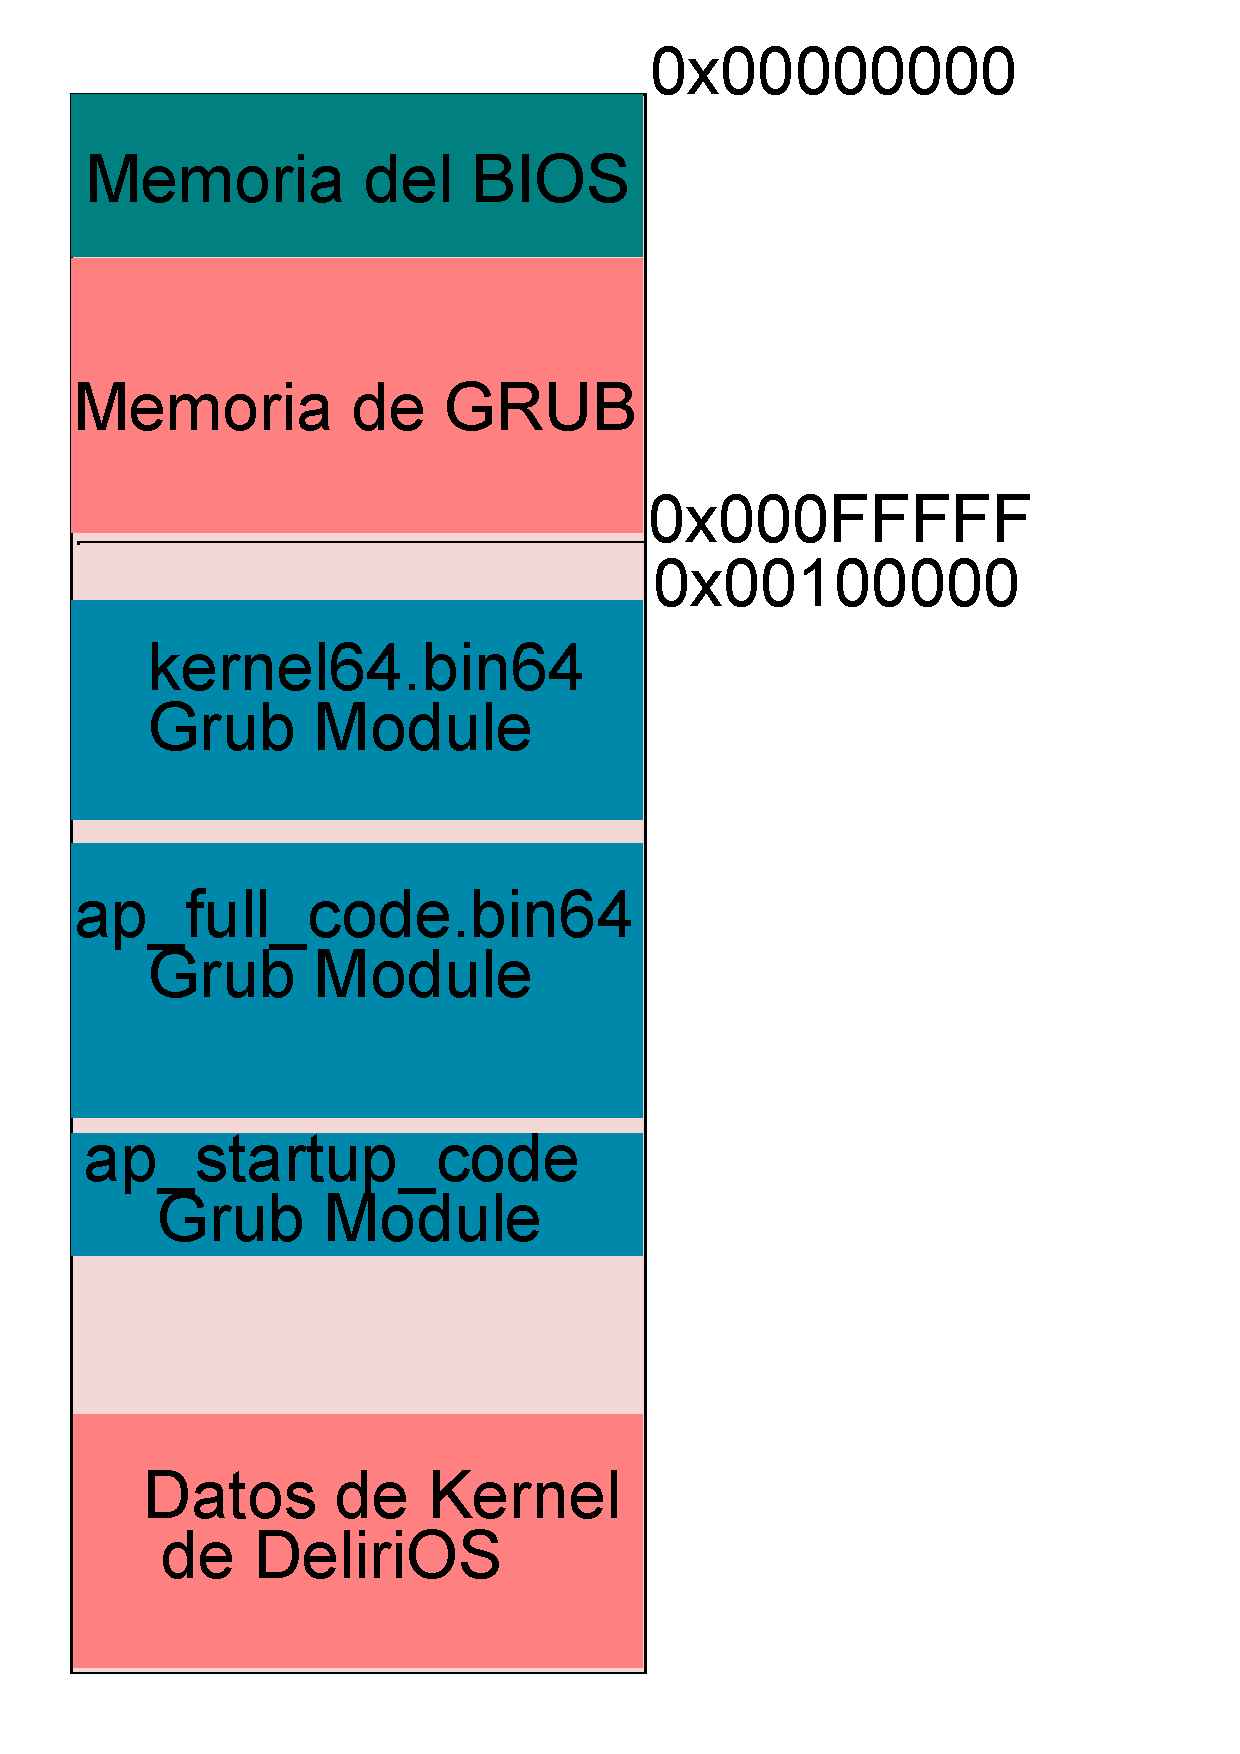
\includegraphics[scale=0.23]{images/modules-map.pdf} 
  \end{center}
\end{frame}

\begin{frame}
  \frametitle{Desarrollo}
  \framesubtitle{Niveles de booteo del BSP y preparación del entorno de inicio de los AP}
  \small Grub inicializa la máquina a un estado conocido y otorga el control al loader de nivel 1 del BSP pasándole por parámetros estructuras de grub con información del sistema.
  \pause
  \begin{enumerate}
  \item Se realizan \textbf{validaciones} requeridas por la especificación multiboot, verificación de firmas, etc.
  \pause
  \item Se obtienen de la metadata provista por \texttt{grub} las posiciones de memoria \textbf{donde están cargados} los módulos, ellos son:
  \vspace{0.1cm}
  \begin{description} \scriptsize
  \item [kernel64.bin64:] \hfill \\ segundo nivel de \textbf{booteo del BSP}\\ (binario plano de 64 bits)
  \item [ap\_full\_code.bin64:] \hfill \\ segundo nivel de \textbf{booteo de los Application Processors}\\ (binario plano de 64 bits)
  \item [ap\_startup\_code:] \hfill \\ código de inicio del \textbf{AP en modo real y el primer stage} de booteo a modo protegido (binario de 32 bits)
  \end{description}
  \end{enumerate}
\end{frame}

\begin{frame}
  \frametitle{Desarrollo}
  \framesubtitle{Niveles de booteo del BSP y preparación del entorno de inicio de los AP (cont...)}
  \begin{enumerate}
    \setlength{\itemsep}{10pt}
   \small
  \item Los AP inician en modo real $\rightarrow$ deben comenzar su ejecución por debajo del primer mega de memoria principal $\rightarrow$
  se copia el módulo \texttt{ap\_startup\_code} a una dirección arbitraria alineada a página \texttt{0x2000}. (se superpone código con \texttt{grub})
  \pause  
  \item Para evitarlo, minimizamos el tamaño del startup de modo real del AP, haciendo lo antes posible un salto a un loader de nivel 2 por encima del mega (\texttt{ap\_full\_code.bin64})
  \pause
  \item El AP debe saltar entre los dos niveles de booteo $\rightarrow$ se le inyecta al primer módulo la dirección donde esta cargado el segundo nivel de booteo
  \pause
  \item Finalmente, se realiza un salto en la ejecución a donde comienza el modulo \texttt{kernel64.bin64} donde el BSP finaliza la inicializacion del contexto hasta modo largo de 64 bits y enciende a los demás núcleos del sistema
  \end{enumerate}
\end{frame}

\begin{frame}
  \frametitle{Desarrollo}
  \framesubtitle{Inicializacion por niveles BSP}
  \begin{center}
  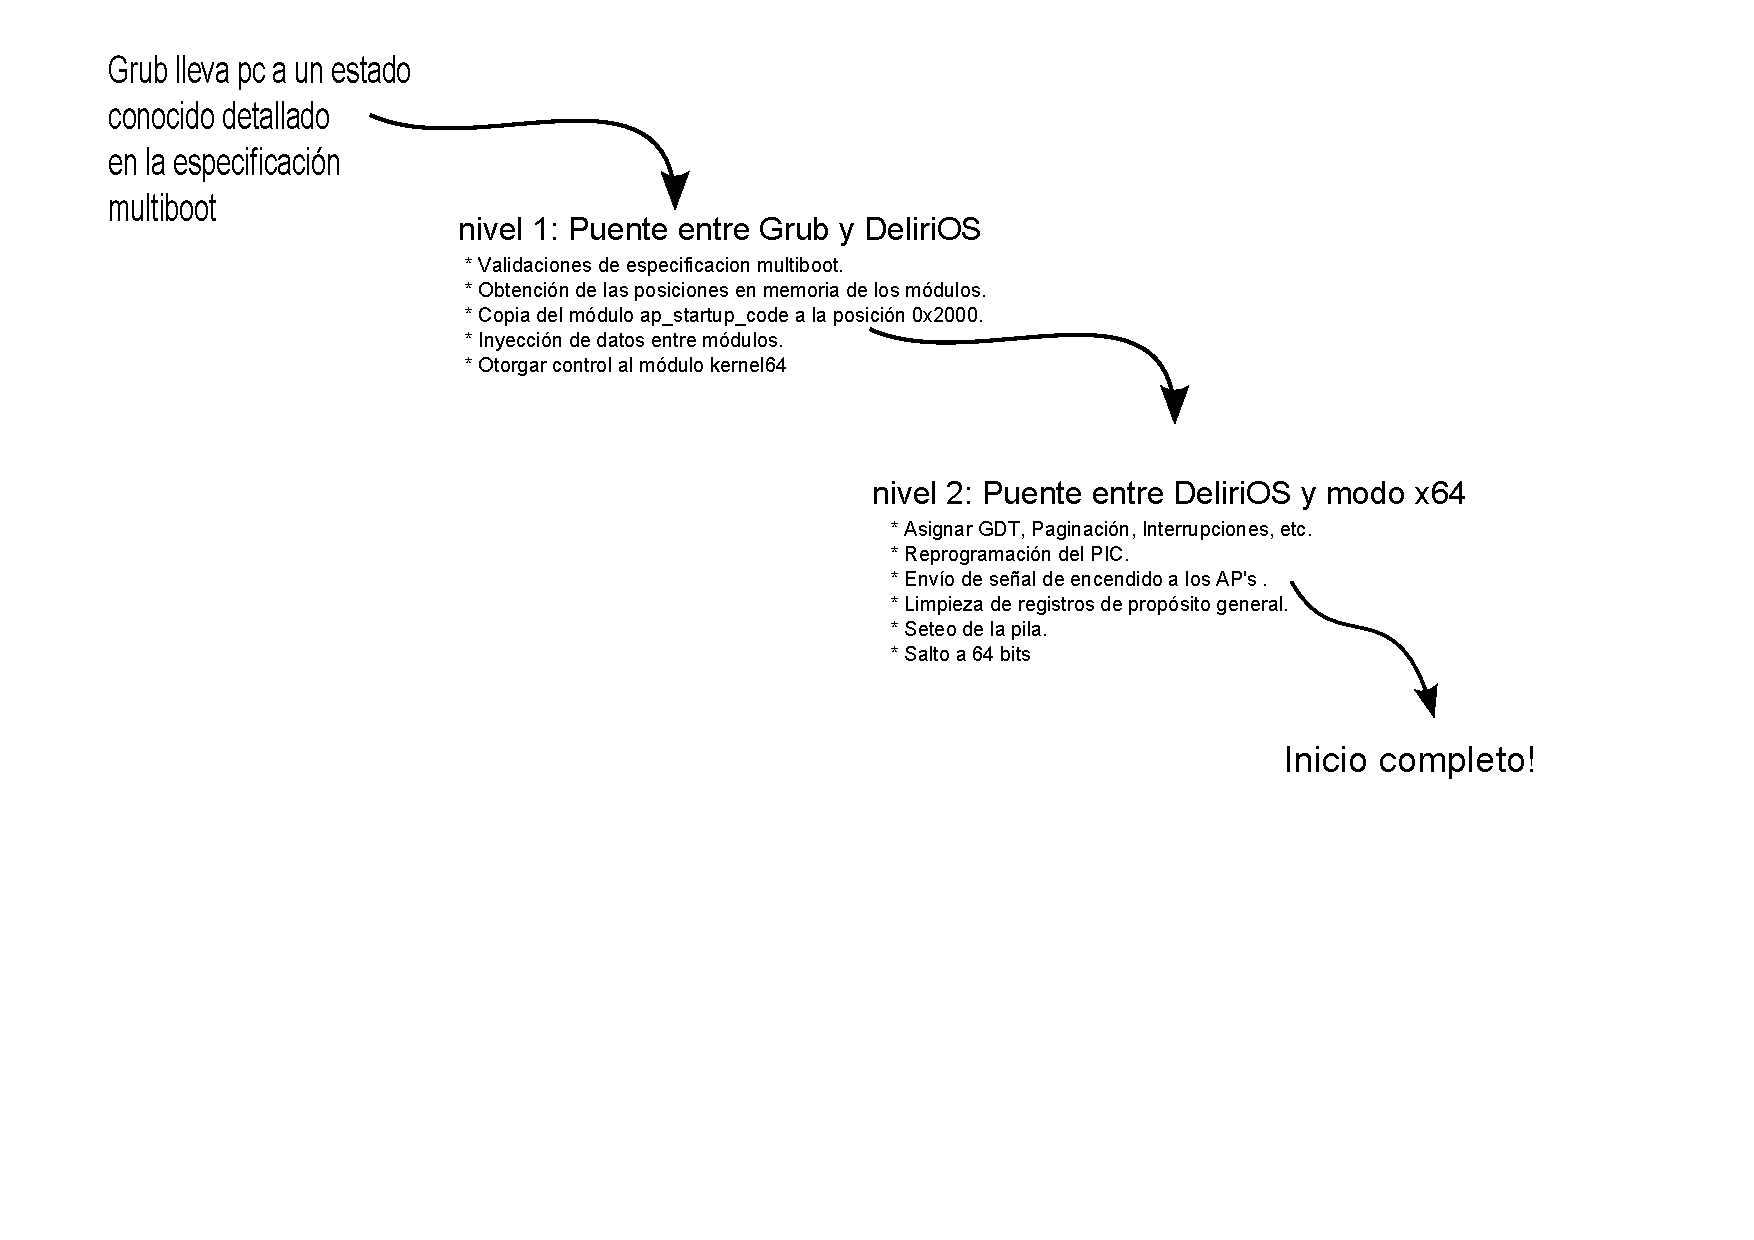
\includegraphics[height=9.5cm]{images/bsp-stages-diagram.pdf} 
  \end{center}
\end{frame}

\begin{frame}
  \frametitle{Desarrollo}
  \framesubtitle{Inicializacion por niveles AP}
  \begin{center}
  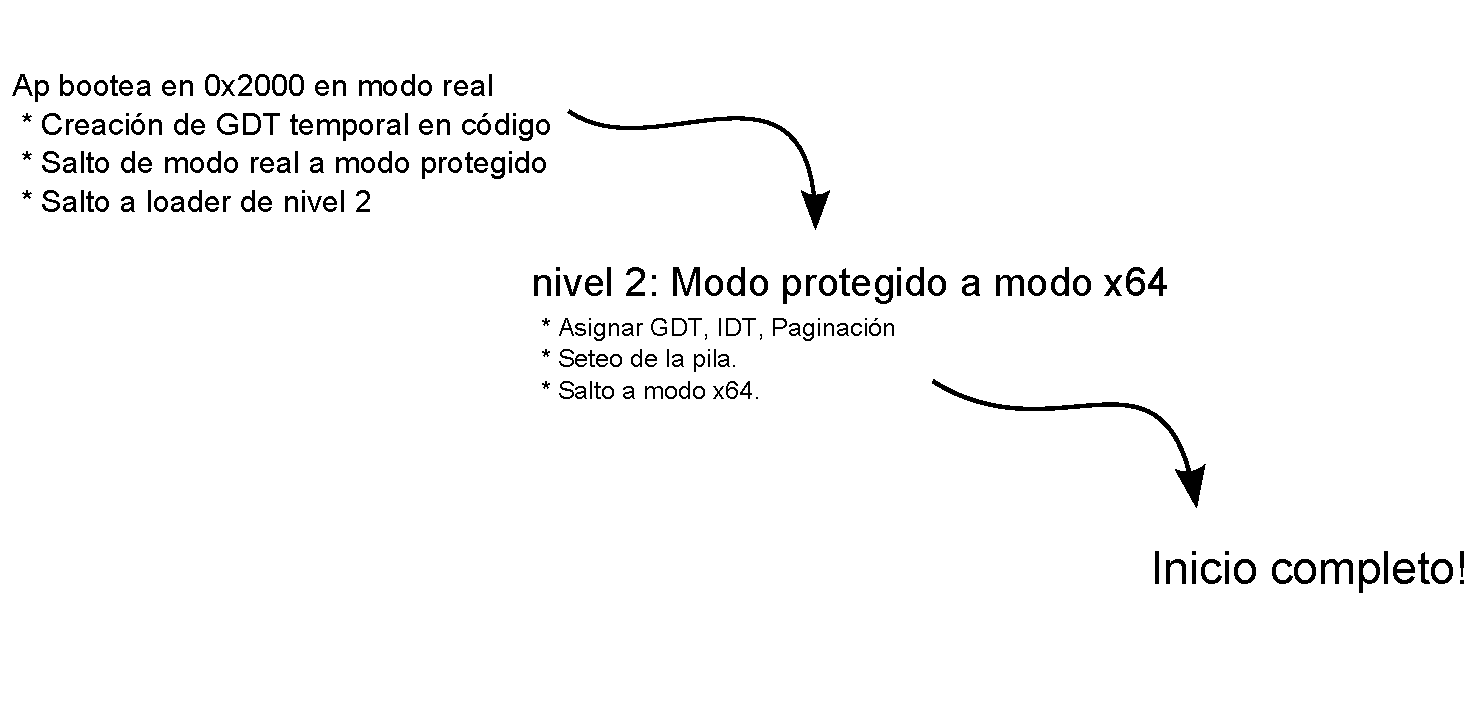
\includegraphics[height=5cm]{images/ap-stages-diagram.pdf} 
  \end{center}
\end{frame}

\begin{frame}
  \frametitle{Desarrollo: Inicialización del Bootstrap Processor} % Pasaje desde modo protegido hacia modo legacy x64
  \framesubtitle{Modo Legacy x64: Modelo de segmentación}
%   \huge \textcolor{red}{QUIEN ASEGURA ??? explicar mejor o detallar en pasos} \\ % TODO
%   \small
%   La especificación \emph{multiboot} nos asegura que estamos en modo protegido, pero no tenemos la certeza de tener asignada una GDT válida, es por esto que asignamos una GDT con 3 descriptores de nivel 0, una para datos y otras dos de código, esta diferenciación de descriptores de código es necesaria para realizar los jump far para pasar de modo real hacia modo protegido y de modo protegido-compatibilidad x64 hacia modo largo x64.
  \small
  La especificación de \emph{multiboot} de \texttt{grub} asegura que estamos en modo protegido\\
  \vspace{0.5cm}
  Pero podemos no tener asignada una GDT válida\\
  \vspace{0.5cm}
  Necesitamos las siguientes entradas en la GDT,
  \vspace{0.5cm}
  \begin{center}
  \begin{tabular}{|c|c|}
  \hline
  Índice & Descriptor\\
  \hline
  0 & Descriptor nulo\\
  \hline
  1 & Código nivel 0 para 32 bits\\
  \hline
  2 & Código nivel 0 para 64 bits\\
  \hline
  3 & Datos nivel 0 para 32 y 64 bits\\
  \hline
  \end{tabular}
  \end{center}
\end{frame}

\begin{frame}
  \frametitle{Desarrollo: Paginación en 64 bits}
  \framesubtitle{x64 requiere habilitar PAE}
%   Como se puede apreciar, tiene mas niveles que la paginacion comun en modo protegido de 32 bits.
  Se realizo un mapeo identity mapping de los primeros 4gb usando paginas de 4kb.
  \begin{center}
  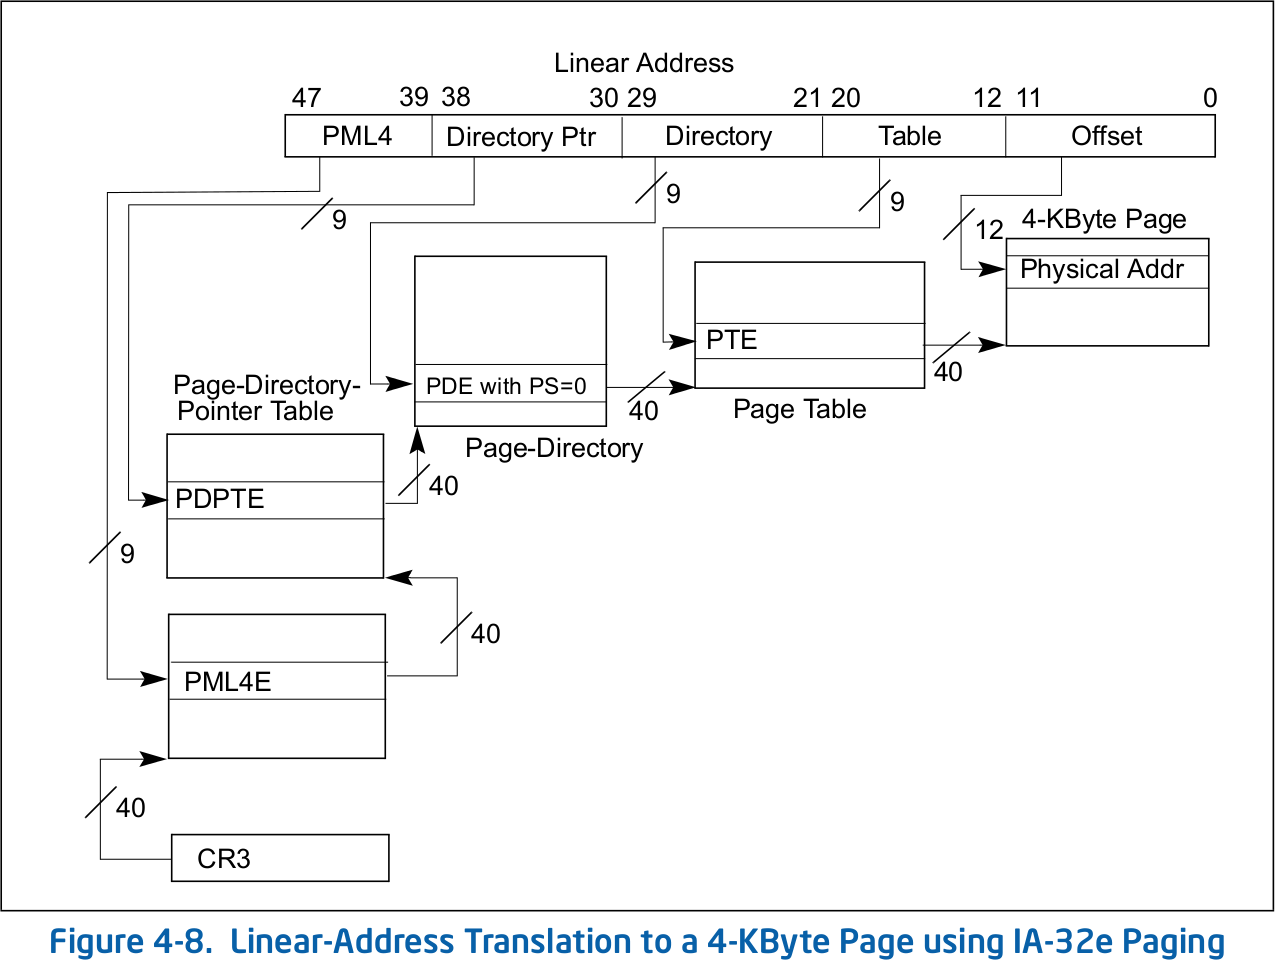
\includegraphics[height=6cm]{images/ia32-paging-overview_INTEL.png} 
  \end{center}
\end{frame}

\begin{frame}
  \frametitle{Desarrollo: Verificacion de disponibilidad de x64}
  \framesubtitle{Consulta via \texttt{cpuid}}
  Luego de establecer estas estructuras, realizamos una comprobación vía \texttt{cpuid} para saber si está disponible modo x64, \\ 
  \vspace{20pt}
  de verificarse esta comprobación, encendemos los bits del procesador correspondientes para habilitar dicho modo en el registro CR0.
\end{frame}

\begin{frame}
  \frametitle{Desarrollo: Pasaje a modo largo x64 nativo}
  Para pasar de modo compatibilidad a modo nativo de 64 bits, es necesario realizar un salto largo en la ejecución a un descriptor de la GDT de código de 64 bits.\\
  \vspace{20pt}
  Luego de realizar el salto al segmento de código de x64 de la GDT establecemos un contexto seguro con los registros en cero, seteamos los selectores correspondientes de la GDT y establecemos los punteros a una pila asignada al BSP.
\end{frame}

\begin{frame}
  \frametitle{Desarrollo: Inicialización del PIC}
  \framesubtitle{Captura de excepciones e interrupciones}
  Enviamos señales al PIC para reprogramarlo de forma tal en la que atienda las interrupciones enmascarables.\\
  \vspace{20pt}
  Luego, asignamos una IDT que captura todas las excepciones e interrupciones y de ser necesario, realiza las acciones correspondientes con su ISR asociada.
%   \\
%   \vspace{20pt}
%   Particularmente las excepciones son capturadas y mostradas en pantalla y se utiliza la interrupción de reloj para sincronización y esperas, las demás interrupciones son ignoradas. \huge \textcolor{red}{esta frase no tiene sentido. o si?}
\end{frame}

% \begin{frame}
% \huge \textcolor{red}{que onda este dibujo? porque esta, que explicacion tiene?}
%   \begin{center}
%   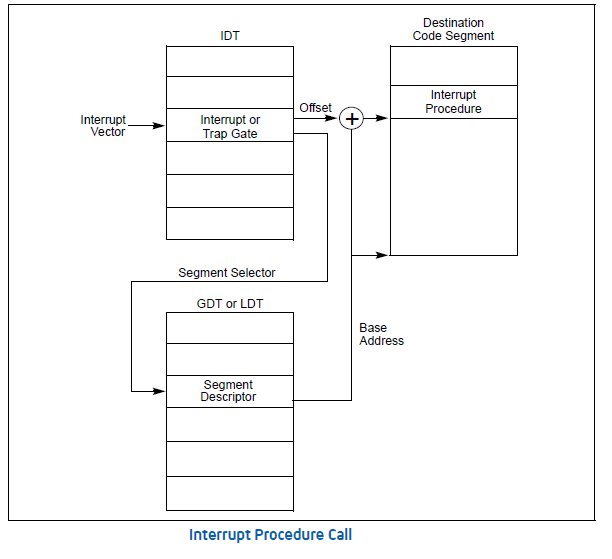
\includegraphics[height=8cm]{images/interrupts.png}
%   \end{center}
% \end{frame}

\begin{frame}
\frametitle{Desarrollo: Multicore - encendido de los AP's}
Una vez inicializado el bsp, se procede a inicializar el resto de los procesadores del sistema.\\
\vspace{20pt}
Para lograr esto, primero es necesario que encontrar una estructura de datos llamada \texttt{MP Floating Pointer Structure}, que contiene:

\begin{itemize} \scriptsize
 \item información sobre los demás procesadores
 \item apic (advanced programable interrupt controller)
 \item el I/O apic (análogo al apic, pero se encarga además de rutear interrupciones de input/output a los lapic's)
\end{itemize}
\end{frame}

\begin{frame}
  \frametitle{Desarrollo: \small Búsqueda de la estructura \texttt{MP Floating Pointer}}
  Esta estructura puede estar en diferentes lugares de memoria, inicialmente se debe realizar la búsqueda dentro del \textbf{primer kilobyte de la ebda} (extended bios data area), \\
  de no encontrarse allí, se procede a buscar entre los \textbf{639K-640K} de memoria.\\
  \vspace{10pt}
  \begin{itemize}
   \item Para encontrar la tabla se busca dentro de esas áreas de memoria la firma de la \texttt{MP Floating Pointer Structure}, la cual es "\texttt{\_MP\_}"
  \item Para comprobar la validez de la estructura se realiza un checksum
  \item Si no se encuentra la tabla, el sistema no soporta multicore
  \end{itemize}
\end{frame}

% \begin{frame} % TODO esto lo saco y lo pongo arriba
%   \frametitle{Desarrollo: \small Comprobación de checksum de la estructura}
%   Una vez encontrada una estructura con esa firma, es necesario realizar una comprobación de checksum para verificar que la misma sea válida.
%   De no ser válida la estructura encontrada, se continúa buscando dentro de las áreas de memoria previamente mencionadas, al agotarse las áreas mencionadas sin éxito en la búsqueda, se concluye que el sistema no soporta multicore.
% \end{frame}

% \begin{frame} % TODO esto lo saco, mucho detalle.
%   \frametitle{Desarrollo: \small Habilitación de ICMR y Local APIC}
%   El sistema luego es configurado usando la MP Configuration Table, extraída de la MP Floating Pointer Structure, que contiene en diferentes entradas la información acerca de los diferentes dispositivos utilizados en multicore.
%   Una vez parseadas estas entradas, si la maquina tiene ICMR, se habilita ese registro, y luego se procede a inicializar el apic local del bsp, seteando el vector de interrupciones espurias (interrupciones por ruido de hardware, etc) y habilitando el bit de enable dentro de los registros del local apic. (Registros del local apic especificados en Table 10-1 Local APIC Register Address Map, manual 3 de intel capitulo 10).
% \end{frame}

\begin{frame}
  \frametitle{Desarrollo: \small Inicialización de los AP's}
  Una vez finalizada la inicialización del \texttt{local apic}, se debe pedir a la BIOS que setee el \texttt{warm reset vector} a la dirección donde esta localizado el inicio de modo real de los aps$(0x2000)$.\\
  \vspace{10pt}
  Luego de este paso, se procede a encender los AP's usando la información obtenida por la \texttt{MP Configuration Table}.
%   El proceso de encendido los aps consiste en preparar 3 estructuras de interrupt command register (registro del apic usado para ipis) para luego enviar las ipis especificas de inicio. El primer icr se setea con el delivery mode de INIT, que sea una interrupción por nivel y con la dirección del ap a iniciar. El segundo icr se setea con el delivery mode de INIT\_DASSERT, que sea una interrupción por flanco, y que sea enviado a todos los procesadores. El tercer icr se setea con el delivery mode STARTUP, la dirección física de la página de inicio de ejecución del ap shifteado 12 a derecha, y la dirección del ap.
\end{frame}

\begin{frame}
  \frametitle{Desarrollo: \small Inicialización de los AP's (cont)}
  Luego de tener listos los \texttt{icr}, se procede a mandar las \texttt{ipi's} de INIT e INIT\_DASSERT, luego se espera unos 10 milisegundos, verificando previamente que las \texttt{ipis} se hayan enviado correctamente. \\
  \vspace{10pt}
  Luego de la espera, se procede a enviar la \texttt{ipi} de STARTUP, se espera 10 ms, se verifica que se haya enviado correctamente, se la vuelve a enviar, se realiza otra espera de 10 ms, y se vuelve a verificar.\\
  \vspace{10pt}
  Una vez terminado este proceso, se puede asumir que el AP fue encendido, y se continúa el encendido el resto de los AP's encontrados en la \texttt{MP Configuration Table}
\end{frame}

% \begin{frame} % TODO: comentenlo hablando
%   \frametitle{Notas}
%   \textbf{Nota 1: } El proceso de inicialización de los aps se encuentra especificado en detalle en el manual de intel volumen 3, capitulo 8, subsección 4, MULTIPLE-PROCESSOR (MP) INITIALIZATION.
% 
%   \textbf{Nota 3: } Los identificadores de núcleo no necesariamente son valores numéricos consecutivos.
% \end{frame}

\begin{frame}
  \frametitle{Desarrollo: \small Inicialización de modo real a modo nativo x64 de los AP's}
%   Como vimos en la sección anterior, los Application Processors comienzan su ejecución en una posición otra por debajo del primer mega en modo real, nosotros necesitamos hacer saltar la ejecución a una posición conocida por encima del mega que no se solape con estructuras del kernel ni otros módulos, la solución que propusimos es un booteo por etapas.
  booteo por etapas,\\
%   \subsubsection{Booteo por niveles: Modo real a modo protegido y modo protegido en memoria alta}
\vspace{10pt}
  \begin{enumerate}
    \setlength{\itemsep}{10pt}
   \item Se inicializa una GDT básica y se salta a modo protegido
   \item Salto al segundo bootloader (dirección inyectada)
   \item Pasamos a modo nativo de 64 bits
   \item Se asignan estructuras comunes, la GDT y la estructura de paginación
   \item Se inicializa una IDT para los AP y se habilitan los local-apic de cada AP
   \item Se obtiene el codigo de identificación del procesador (variable y distinto)
  \end{enumerate}

%   En este primer nivel el núcleo se encuentra en modo real, se inicializa una GDT básica en el mismo código y se salta a modo protegido, esto es necesario para poder direccionar posiciones de memoria por encima del primer mega.\\
%   Recordando secciones anteriores, cuando el BSP iniciaba el primer nivel de booteo preparaba el contexto de los APS para inicializar en niveles, en este proceso se inyecta en el código del primer nivel de booteo del AP la posicion de memoria donde esta el segundo nivel de booteo por encima del mega.\\
%   Luego resta únicamente realizar el salto al segundo bootloader con un jump para continuar el booteo del AP, de manera similar al BSP pasamos luego a modo nativo de 64 bits.\\
%   Notemos que por ejemplo la línea A20 ya esta habilitada, y algunas estructuras del kernel que fueron inicializadas por el BSP son comúnes a todos los núcleos, como por ejemplo la GDT y la estructura jerárquica de paginación, que son directamente asignadas a los registros del núcleo correspondiente con punteros a ellas.\\
%   Para el manejo de interrupciones y excepciones, se inicializa una IDT para los Application Processors, además es necesario habilitar los local-apic de cada AP, en caso contrario, no podríamos utilizar interrupciones inter-procesador(IPIS).\\
%   Como el número de application processors puede ser variable a priori, cuando un núcleo comienza su ejecución, es obtenido su código de identificación dentro del procesador y luego se obtiene una posición de memoria única para cada núcleo con el fin de poder asignar los punteros de la pila $RSP$ y $RBP$, de ser necesaria la reserva de memoria para alguna otra estructura única por núcleo se puede utilizar este recurso.
\end{frame}

\section{Experimentos}

\begin{frame}
  \frametitle{Experimentos: Sorting Paralelo}
  Combinando \emph{merge sort} con \emph{heap sort} se construyo un algoritmo de ordenamiento en paralelo\\
%   Se optó en este caso por un algoritmo propio que combinara varios ordenamientos conocidos con el objetivo de hacer mas fácil la paralelización del experimento. En particular lo que se realiza es partir el arreglo en 2 mitades, donde cada core realiza heapsort sobre su mitad asignada y luego una intercalación de los resultados con un algoritmo también paralelo en el cual un core realiza el merge de los máximos y el otro el merge de los mínimos, luego resta copiar los resultados y concluimos.
  \vspace{10pt}
  El algoritmo tiene 3 subprocesos,\\
  \vspace{10pt}
  \begin{itemize}
  \item Sort: Ordenamiento de mitades por cada core
  \item Merge: Merge paralelizado de las mitades ordenadas
  \item Copy: Copia del resultado a un buffer de destino
  \end{itemize}
  \vspace{10pt}
  Dos mecanismos de sincronización,\\
  \vspace{10pt}
  \begin{itemize}
  \item Memoria: \emph{Polling} sobre memoria
  \item Ipis: interrupciones entre procesadores
  \end{itemize}
\end{frame}

% \begin{frame}
%   \frametitle{Experimentos: Memoria}
%   \begin{center}
%   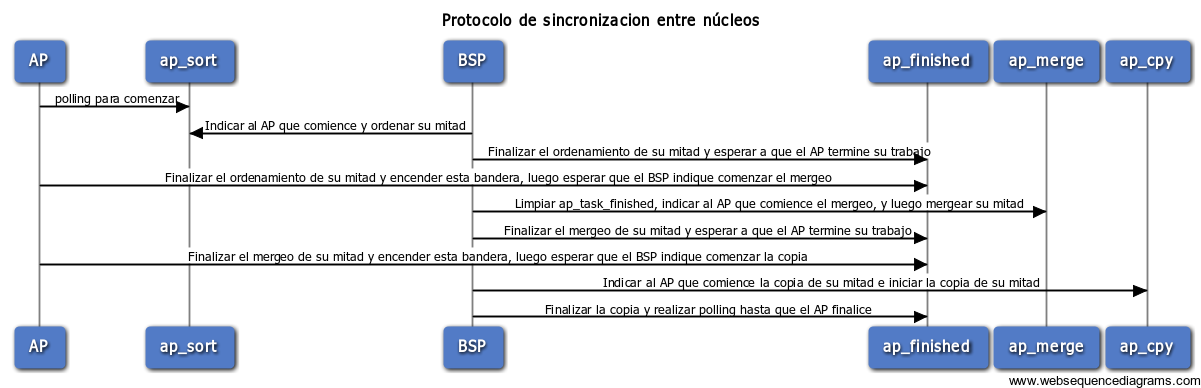
\includegraphics[scale=0.28]{images/sync-sorting-seq.png}
%   \end{center}
% \end{frame}
% 
% \begin{frame}
%   \frametitle{Experimentos: Ipis}
%   \begin{center}
%   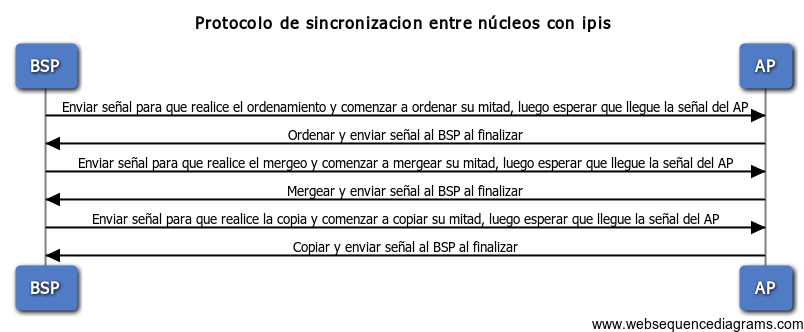
\includegraphics[height=4.5cm]{images/ipis-sorting-seq.png}
%   \end{center}
% \end{frame}

% \begin{frame}
%   \frametitle{Resultados}
%   \framesubtitle{Intel® Pentium® Processor G2030 - Sorting}
%   \begin{center}
%   \begin{tabular}{|c|c|c|c|c|c|c|}
%   \hline	
%   Elementos & Ratio Mem/Ipi & Single/DMem & Single/DIpi\\
%   \hline
%   2 & 0.213 & 0.705 &  0.150\\
%   \hline
%   4 & 0.291 & 0.929 &  0.270\\
%   \hline
%   8 & 0.375 & 1.422 &  0.534\\
%   \hline
%   16 & 0.564 & 1.634 &  0.923\\
%   \hline
%   32 & 0.682 & 1.879 &  1.283\\
%   \hline
%   64 & 0.833 & 1.944 &  1.619\\
%   \hline
%   128 & 0.923 & 1.96 &  1.810\\
%   \hline
%   512 & 0.967 & 2.037 &  1.971\\
%   \hline
%   131072 & 0.987 & 2.024 &  1.999\\
%   \hline
%   262144 & 0.991 & 2.095 &  2.077\\
%   \hline
%   524288 & 0.989 & 2.029 &  2.008\\
%   \hline
%   1048576 & 0.992 & 2.018 &  2.003\\
%   \hline
%   2097152 & 0.989 & 2.034 &  2.013\\
%   \hline
%   4194304 & 0.994 & 2.023 &  2.012\\
%   \hline
%   \end{tabular}
%   \end{center}
% \end{frame}

\begin{frame}
  \frametitle{Experimentos: Sorting Paralelo}
  \framesubtitle{Resultados en un procesador G2030}
  \begin{center}
  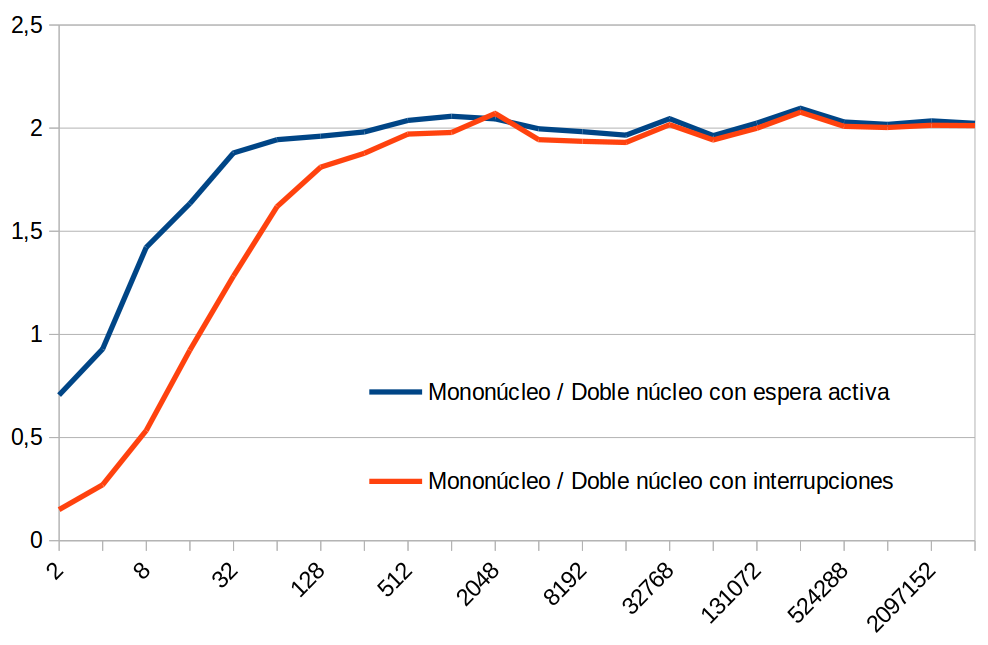
\includegraphics[scale=0.3]{images/grafico.png}
  \end{center}
\end{frame}

\begin{frame}
  \begin{center}
  \huge GRACIAS
  \end{center}
\end{frame}

\end{document}